\section{Mathematical modelling}
\label{chap1:sec:mathematical_modelling}

The physical phenomena involved in the polymer processing applications of interest are mathematically modelled in the present section such that the computational modelling approach can be applied, for which the extrusion process is taken as an example.
In that regard, the mathematical models derive from several theories, namely the rheology to provide the constitutive equations for the constitutive modelling of polymeric fluids, and the fluid mechanics to provide the governing equations for the heat and mass transfer modelling.
A comprehensive description of the mathematical modelling of polymeric fluid flows is found, for instance, in the books of R.B. Bird et al., 1987~\cite{chap1:1987bird}, C.W. Macosko, 1994~\cite{chap1:1994macosko}, R.G. Larson, 1999~\cite{chap1:1999larson}, and F.A. Morrison, 2011~\cite{chap1:2001morrison}, which is briefly described as hereafter.

\subsection{Constitutive modelling}
\label{chap1:subsec:computational_modelling_rheology_modelling}

The rheology is a well-established science for a wide range of materials, particularly polymeric materials, dedicated to the study of deformation and fluid flow involving a viscous or viscoelastic response to stress.
Constitutive equations for polymeric fluids are often based in rheological principles to describe the phenomenological relationships between mechanical variables (and eventually also thermal variables) mathematically.
Newton's law of viscosity states that the stress of a fluid in motion changes linearly with the strain rate, where the proportionality constant is referred to as dynamic or absolute viscosity.
Many examples of these Newtonian fluids are present everywhere, such as water, mineral oil, and gas.
However, the complex nature of polymers makes the stress in polymeric fluid flows exhibit a non-trivial response to the strain rate, usually significantly deviating from Newton's law of viscosity.
In that regard, more complex constitutive equations for these non-Newtonian fluids are needed, often derived from empirical relations within experimentation rather than based on fundamental physical principles.

Several theories for the rheology of non-Newtonian fluids attempt to adequately describe the non-trivial behaviour of polymeric fluids, providing constitutive models that gradually increase in complexity.
The most straightforward approach is the generalized Newtonian fluid, which consists in replacing the absolute viscosity with an apparent or effective viscosity, which is a function of the second invariant of the strain rate tensor.
Empirical relations, such as the classical power-law, are then used to quantitatively describe the non-linear response of the stress to the strain rate, for which experiments are required to determine the characteristic parameters in the empirical constitutive relation for the fluid.
The generalized Newtonian fluid approach becomes convenient and straightforward, providing valid results in a variety of applications, particularly those comprising slow processes, when comparing the process characteristic time with the material relaxation time.
Many non-Newtonian fluids exhibiting different behaviours are appropriately modelled as generalized Newtonian fluids.
For instance, shear-thinning or shear-thickening fluids, where increasing stress leads to the decrease and increase of the apparent viscosity, respectively.
Another example is thixotropic and rheopecty fluids, showing a time-dependent viscous change, where the duration of the applied stress decreases and increases the apparent viscosity, respectively.
However, since the strain rate history is not considered, the generalized Newtonian fluid approach only reproduces a viscous response, also referred to as inelastic, whereas polymeric fluids exhibit a combination of viscous and elastic responses.
Consequently, the generalized Newtonian fluid approach might inadequately describe the behaviour of these fluids in polymer processing applications.

The constitutive modelling for viscoelastic responses consists in splitting the stress tensor into a solvent contribution and a polymer solute contribution, also referred to as elastic or polymeric stress.
The solvent is assumed to have a Newtonian behaviour, whereas the polymer solute requires complex partial differential equations that comprise several relaxation modes, due to the length distribution of the polymer chains.
From linear to non-linear viscoelastic fluids, several constitutive models attempt to reproduce better the observed behaviour of complex polymeric fluids, which unfortunately comes at the cost of increasing complexity.
Examples of empirical relations for the constitutive modelling of fluids are provided in Figure~\ref{chap1:fig:mathematical_modelling_classification_of_fluids}.
For the sake of completeness, inviscid fluids are mentioned, corresponding to those having a null viscosity and, consequently, no stress, and are of interest in other contexts, such as aerospace applications.

\begin{figure}[!htb]
\centering
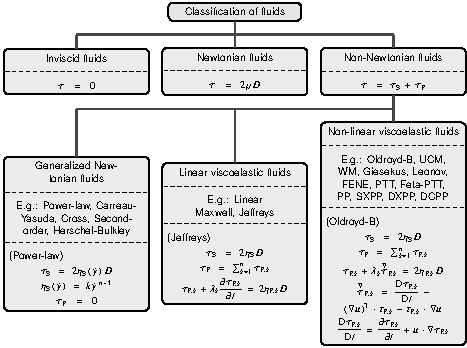
\includegraphics[width=\textwidth]{chap1/include/tikz/classification_of_fluids.pdf}
\caption{Classification and constitutive modelling of fluids.}
\label{chap1:fig:mathematical_modelling_classification_of_fluids}
\end{figure}

\subsection{Heat and mass transfer modelling}
\label{chap1:subsec:computational_modelling_mass_transfer_modelling}

Besides the constitutive modelling of the polymeric fluids in polymer processing applications, the extrusion process consists of two fundamental physical phenomena, namely the heat and mass transfer.
Governing equations for the heat and mass transfer are required, usually involving several physical variables, namely the temperature, velocity, pressure, and stress, whereas the density is also considered in compressible fluid flows.
In that context, the computational fluid dynamics has emerged as a branch of the computational modelling dedicated to the heat and mass transfer modelling in fluid flow problems.
For fluids with non-Newtonian behaviour, such as polymeric fluids, which require complex constitutive equations derived from the rheology theory, this field is often referred to as the computational rheology.

The compressibility effects during the extrusion process, for instance, considering the molten polymeric material flowing through the die, can be neglected and, therefore, the density is a physical property rather than a physical variable.
Moreover, the extrusion process is continuous, and the physical variables do not usually change over time and, therefore, a steady-state situation can be considered.
In that regard, the governing equations for the heat and mass transfer consist of a heat equation, a momentum equation, and a continuity equation, which are illustrated in Figure~\ref{chap1:fig:mathematical_modelling_governing_equations} ($T$ is the temperature, $\bm{u}$ is the velocity, $p$ is the pressure, $\bs{\tau}$ is the stress, $\bm{I}$ is the identity matrix, $\kappa$ is the thermal conductivity, $\rho$ is the density, $c_{\textrm{P}}$ is the specific heat capacity, and $\mu$ is the absolute viscosity).

\begin{figure}[!htb]
\centering
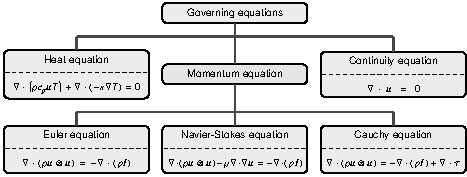
\includegraphics[width=\textwidth]{chap1/include/tikz/governing_equations.pdf}
\caption{Governing equations for steady-state incompressible flows.}
\label{chap1:fig:mathematical_modelling_governing_equations}
\end{figure}

The mass transfer applies only to fluids and requires two governing equations, one for the conservation of mass and another for the balance of momentum of the fluid, also referred to as continuity and momentum equations, respectively.
The continuity equation imposes a null divergence velocity, which guarantees conservation of mass in the system for incompressible fluid flows, whereas the choice of the momentum equation mainly depends on the fluid.
The Euler equation involves only the velocity and the pressure to describes the balance of momentum in inviscid fluid flows and, therefore, is not appropriate to polymer processing applications.
On the other side, the Navier-Stokes equation is usually used to describe the balance of momentum in Newtonian fluid flows, providing the absolute viscosity of the fluid.
For non-Newtonian fluid flows, the Cauchy equation has to be used instead, which becomes more complicated since the contribution of the stress is required in the momentum equation, obtained from the corresponding constitutive equations for the fluid.
However, when the constitutive modelling is provided with explicit empirical relations, as for generalized Newtonian fluids, the contribution of the stress can be rewritten in terms of the effective viscosity, which becomes similar to the Navier-Stokes equation.

From the mass transfer modelling viewpoint, explicit relations between stress and strain rate lead to a model consisting of the Navier-Stokes equation and the continuity equation.
On the other side, implicit relations require the use of the Cauchy equation and, consequently, the stress has to be determined from the constitutive equations that are part of the model.
Moreover, the constitutive modelling often consists of several equations, which in turn unfold into more equations since they are usually written in the tensor form but are solved for each tensor component.
For instance, assuming a tridimensional problem, the momentum equation unfolds into three equations derived for each velocity component, whereas the continuity equation is already in the scalar form.
On the other hand, each constitutive equation unfolds into six equations, assuming a symmetric stress tensor, or nine equations otherwise.
Therefore, the use of implicit constitutive models increases considerably the complexity of the mass transfer modelling, which ultimately raises essential challenges from the numerical and computational viewpoints.

The heat transfer equation describes the energy transport in a solid or fluid material, which occurs through convection and conduction, whereas radiation is usually neglected in polymer processing applications, such as extrusion and injection moulding.
The heat transfer by convection is associated with the motion of mass and, therefore, applies to molten polymeric materials and also to moving parts of the extrusion machine.
The heat convection is proportional to the temperature and the velocity, which are both physical variables of the problem, and also to the density and the specific heat capacity, which are physical properties of the material.
On the other side, the heat transfer by conduction is associated with the random propagation of the microscopic motion of molecules or atoms in favour of decreasing temperature gradients.
In that case, the thermal conductivity of the material measures the associated rate of heat transfer.
Thus, the heat conduction applies not only to molten polymeric materials and moving parts of the extrusion machine but also to all components, such as the cooling/calibration system.

The heat transfer equation can only be solved after the solution of the balance of momentum and continuity equations since the convective transport of energy depends on the velocity.
However, in practice, the opposite is also valid as the physical variables for the mass transfer, namely the density and the viscosity or associated constitutive equations for the material, often depend on the temperature.
Indeed, changes in the physical state also occur during the extrusion process, from the raw polymeric material melting inside the barrel to the final product solidification at the cooling/calibration system.
In that regard, large temperature variations throughout the process are required, making the dependency of these physical properties on the temperature more relevant.
Additionally, the thermal viscous dissipation is another relevant phenomena in polymer processing applications resulting from the typically high stress, which transforms mechanical energy into thermal energy.
In practical terms, the thermal aspects in the extrusion process are relevant for an appropriate mathematical model.
Therefore, the mathematical modelling for polymer processing applications results in non-linear systems of partial differential equations, which cannot be solved for each equation separately.

Boundary conditions complement the governing equations, constraining the physical phenomena on the boundaries of the problem, such as the temperature, the conductive heat flux, the velocity, among others.
Indeed, several types of boundary conditions can be prescribed for the heat and mass transfer, where few examples are illustrated in Figure~\ref{chap1:fig:mathematical_modelling_calibrator_boundary_conditions}, for the mathematical modelling of a cooling/calibration system in the extrusion.
Moreover, interface conditions are required to impose the interaction between different regions in contact, for instance, between the molten polymeric material and the cooling/calibrator system.
In the case of the heat transfer, both the continuity of the temperature and the conservation of the conductive heat flux are usually prescribed, providing valid results in a variety of situations.
However, this idealization of a perfect thermal is not appropriate in many applications since realistic contacts are often composed of microscopic air pockets due to the surface roughness, particularly in solids, as illustrated in Figure~\ref{chap1:fig:mathematical_modelling_surface_roughness}.
In these imperfect thermal contacts, a relevant interfacial thermal resistance arises, which hampers the heat exchange between the polymer melt and the metallic parts.
In that case, temperature jumps are experimentally measured on the interface, as in the case between the molten polymeric material and the cooling/calibration system in the extrusion.
Therefore, specific interface conditions are required to replicate this behaviour appropriately.
This whole range of issues in the extrusion process highlights the importance of properly accounting for the thermal effects in the computational modelling of polymer processing applications.

\begin{figure}[!htp]
\centering
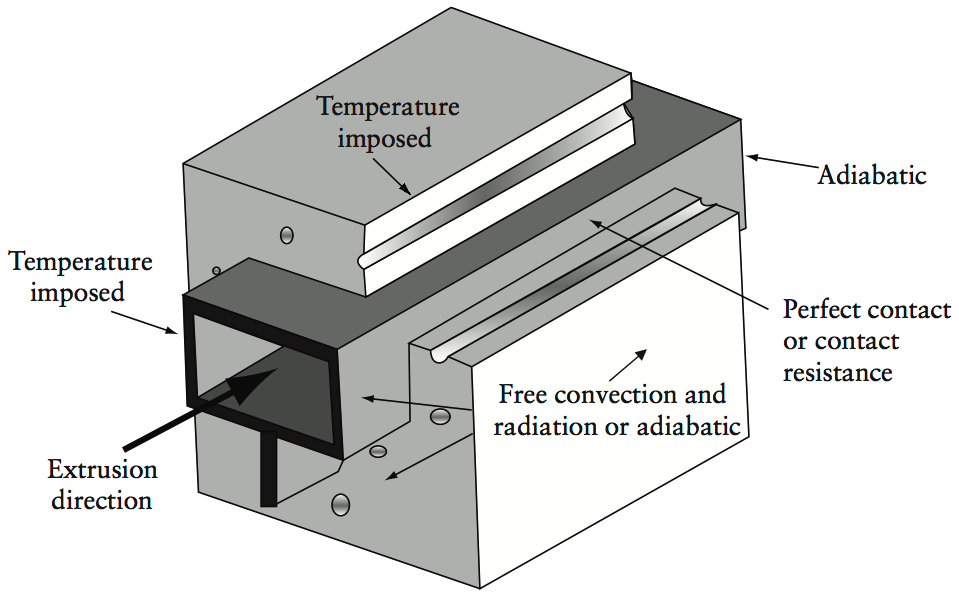
\includegraphics[width=0.7\textwidth]{chap1/include/figures/calibrator2.png}
\caption[Boundary and interface conditions prescribed for the thermoplastic profile extrusion cooling stage with a cooling/calibrator system.]{Boundary and interface conditions prescribed for the thermoplastic profile extrusion cooling stage with a cooling/calibrator system (adapted from O.S. Carneiro, J.M. N\'obrega, Design of extrusion forming tools, Smithers Rapra, Shawbury, 2012).}
\label{chap1:fig:mathematical_modelling_calibrator_boundary_conditions}
\end{figure}

\begin{figure}[!htb]
\centering
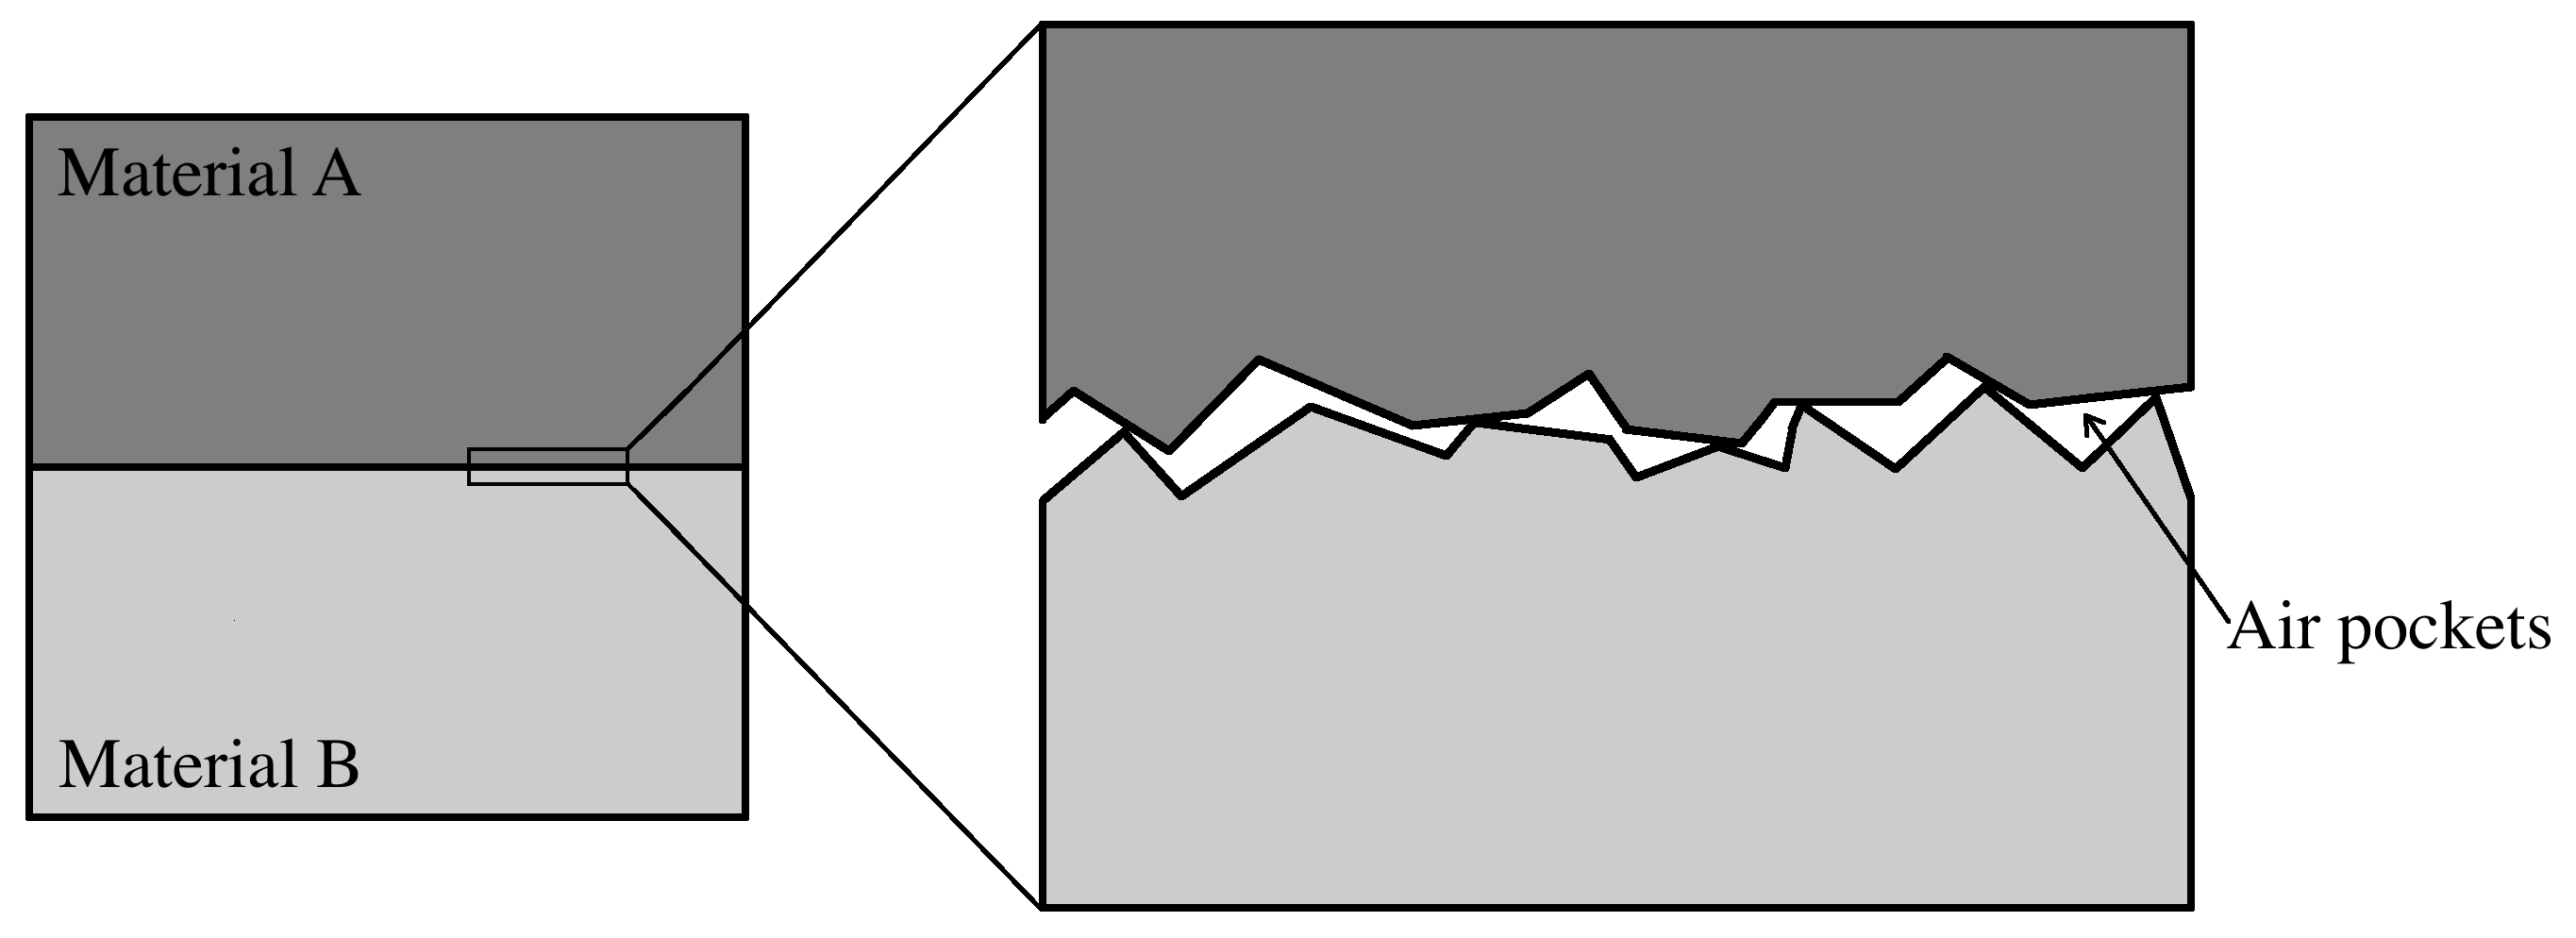
\includegraphics[width=0.7\textwidth]{chap1/include/figures/surface_roughness.png}
\caption{Enlargement of the contact at the microscale between two materials.}
\label{chap1:fig:mathematical_modelling_surface_roughness}
\end{figure}

% end file
